\section{Hyperparameter}
\label{section:hyperparameter}
\begin{table}[t]
	\centering
	\begin{tabular}{l p{0.5\textwidth} l}
		\toprule
		Symbol        & Erklärung                                                                   & Standardwert\\\midrule
		$n_{ep}$      & Anzahl der Schritte in einer Episode                                        & $500$\\
		$p_{max}$     & maximal wählbarer Preis für beide Agenten                                   & $10$\\
		$p_{einkauf}$ & Einkaufs- oder Produktionspreis für Neuprodukte                             & $3$\\
		$p_{lager}$   & Preis pro eingelagertem Gebrauchtprodukt pro Schritt                        & $0.1$\\
		$k$           & Kundenzahl, die pro Schritt den Markt besucht                               & $20$\\
		$m_{lager}$   & maximale Anzahl von Gebrauchtprodukten, die im Lager gehalten werden können & $100$\\
		$c$           & Anteil der Eigentümer, die pro Schritt einen Rückverkauf erwägen            & $0.05$\\\bottomrule
	\end{tabular}
	\caption{Marktparameters mit kurzer Erklärung und für diese Experimente verwendete Standardwerte}
	\label{tab:default_parameters}
\end{table}

\begin{table}[t]
	\centering
	\begin{tabular}{p{0.5\textwidth} l}
		\toprule
		Parameter                                     & Wert\\\midrule
		Lernrate                                      & $10^{-3}$\\
		Größe des Experiencebuffers                   & $10^6$\\
		Episoden bis zum Beginn des Lernens           & $100$\\
		Größe eines Minibatches                       & $100$\\
		Koeffizient für die Polyak-Mittelung ($\tau$) & $0.005$\\
		Diskontierungsfaktor ($\gamma$)               & $0.99$\\\bottomrule
	\end{tabular}
	\caption{Hyperparameter für DDPG und TD3}
	\label{tab:DDPGHyperparameters}
\end{table}

\begin{table}[t]
	\centering
	\begin{tabular}{p{0.5\textwidth} l}
		\toprule
		Parameter                                     & Wert\\\midrule
		Lernrate                                      & $7\cdot 10^{-4}$\\
		Anzahl der Schritte pro Update                & $5$\\
		Diskontierungsfaktor ($\gamma$)               & $0.99$\\\bottomrule
	\end{tabular}
	\caption{Hyperparameter für Advantage Actor Critic}
	\label{tab:A2CHyperparameter}
\end{table}

\begin{table}[t]
	\centering
	\begin{tabular}{p{0.5\textwidth} l}
		\toprule
		Parameter                                     & Wert\\\midrule
		Lernrate                                      & $3 \cdot 10^{-4}$\\
		Anzahl der Schritte pro Update                & $2048$\\
		Größe eines Minibatches                       & $64$\\\
		Anzahl der Epochen pro Update                 & $10$\\
		\textit{clip\_range} ($\varepsilon$)          & $0.2$\\
		Diskontierungsfaktor ($\gamma$)               & $0.99$\\\bottomrule
	\end{tabular}
	\caption{Hyperparameter Proximal Policy Optimization}
	\label{tab:PPOHyperparameters}
\end{table}

\begin{table}[t]
	\centering
	\begin{tabular}{p{0.5\textwidth} l}
		\toprule
		Parameter                                     & Wert\\\midrule
		Lernrate                                      & $3 \cdot 10^{-4}$\\
		Größe des Experiencebuffers                   & $10^6$\\
		Episoden bis zum Beginn des Lernens           & $100$\\
		Größe eines Minibatches                       & $256$\\\
		Entropiekoeffizient ($\alpha$)                & automatisch\\
		Koeffizient für die Polyak-Mittelung ($\tau$) & $0.005$\\
		Diskontierungsfaktor ($\gamma$)               & $0.99$\\\bottomrule
	\end{tabular}
	\caption{Hyperparameter Soft Actor Critic}
	\label{tab:SACHyperparameters}
\end{table}

\section{Definition der regelbasierten Strategien}
\label{section:rulebased_definition}
Der Neupreis wird als
\begin{equation}
	\pi\left(p_{2, neu}\right)_{neu} = \max{\left(p_{2, neu} - 1, p_{einkauf} + 1\right)}
\end{equation}
gesetzt.
Beim Gebraucht- und Rückkaufpreis wird je nach Lagerstand entschieden.
Der Gebrauchtpreis wird in Abhängigkeit des Konkurrenzpreises und des Lagerstandes folgendermaßen gesetzt:
\begin{equation}
	\pi\left(p_{2, gebraucht}, n_{lager}\right)_{gebraucht} =
	\begin{cases}
		p_{2, gebraucht} + 1 & n_{lager} < m_{lager} / 15\\
		p_{2, gebraucht} - 1 & n_{lager} < m_{lager} / 8\\
		p_{2, gebraucht} - 2 & \text{sonst}
	\end{cases}
\end{equation}
Beim Rückkaufpreis werden die gleichen Fallunterscheidungen unternommen und der Preis gesetzt als:
\begin{equation}
	\pi(p_{2, re}, n_{lager})_{re} =
	\begin{cases}
		p_{2, re} + 1 & n_{lager} < m_{lager} / 15\\
		p_{2, re} - 1 & n_{lager} < m_{lager} / 8\\
		p_{2, re} - 2 & \text{Sonst}
	\end{cases}
\end{equation}
Alle Preise werden auf den Aktionsraum beschränkt (für den Fall, dass die Rechnung Ergebnisse kleiner als null oder größer als $p_{max}$ ermittelt).

\section{Weitere Diagramme zum Lernerfolg}
\begin{figure}[htbp]
	\centering
	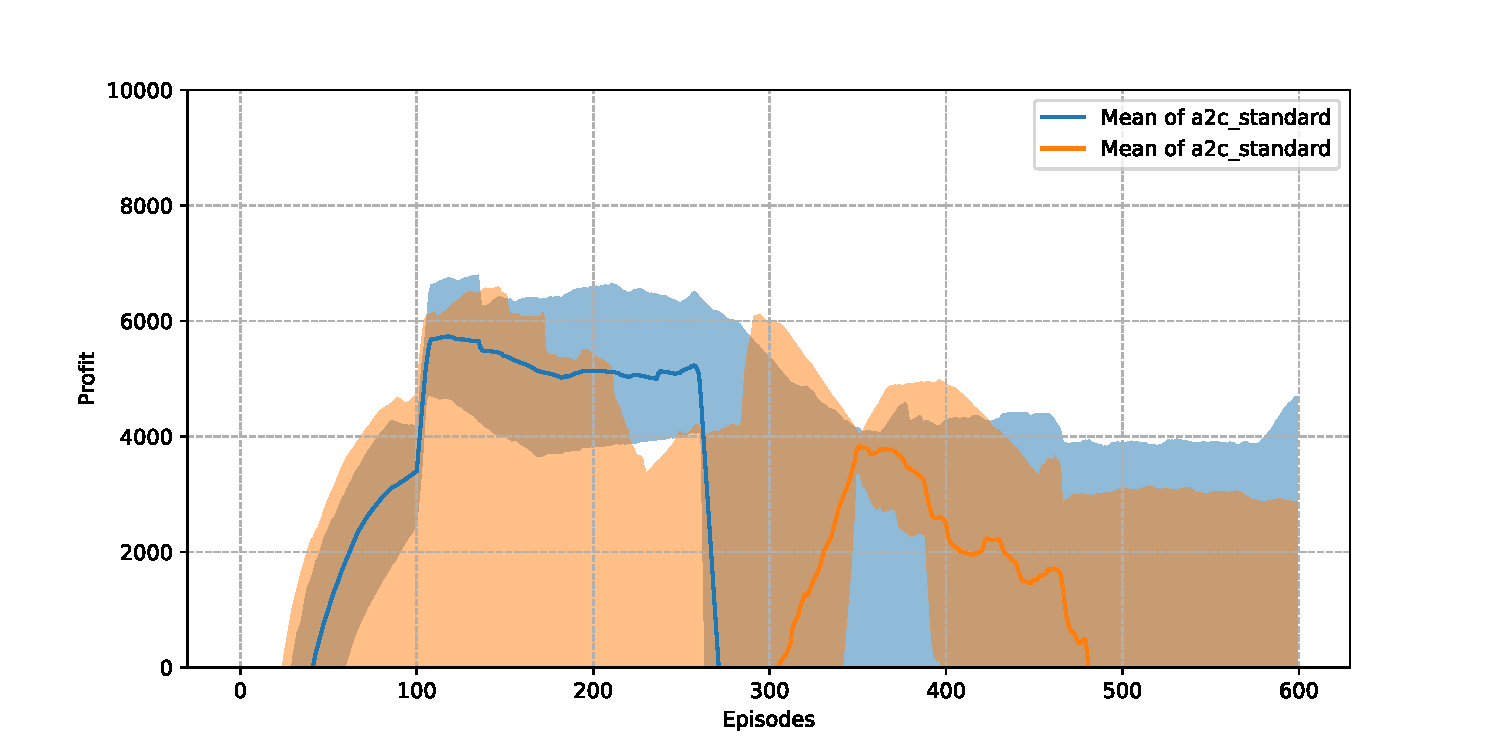
\includegraphics[width=\textwidth]{appendix/mixed_rewards_a2c.pdf}
	\caption{
		Lernkurve des Advantage-Actor-Critic-Algorithmus bei gemischter Rewardfunktion (orage) im Vergleich zur Standardfunktion (blau):
		Man sieht, dass einige Durchläufe mit gemischter Rewardfunktion einen ähnlichen Verlauf nehmen wie die mit Standardrewardfunktion.
		Andere Läufe machen kaum Gewinn und leiden unter sehr viel Instabilität.
	}
	\label{graphic:MixedRewardsA2C}
\end{figure}
\begin{figure}[htbp]
	\centering
	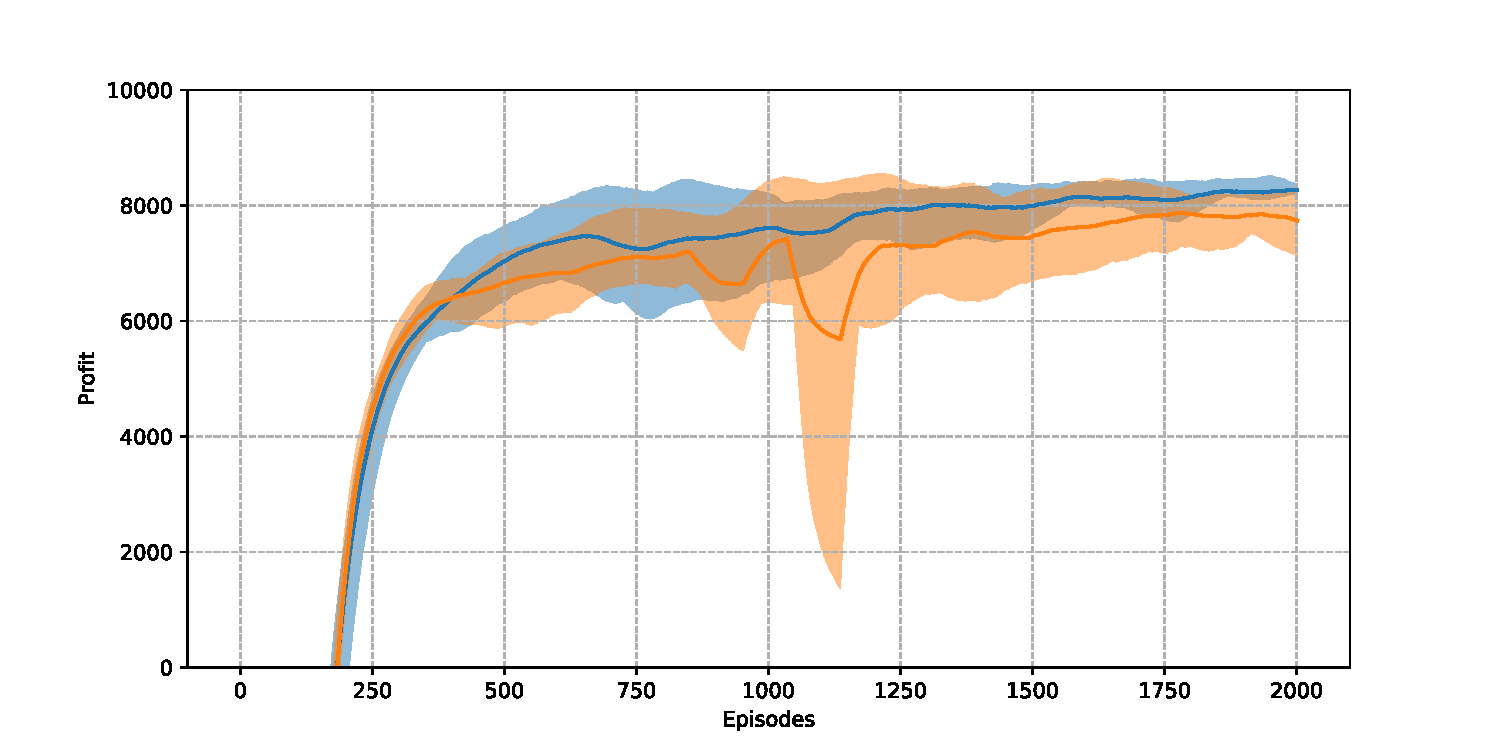
\includegraphics[width=\textwidth]{appendix/mixed_rewards_ppo.pdf}
	\caption{
		Lernkurve des Proximal-Policy-Optimization-Algorithmus bei gemischter Rewardfunktion (orage) im Vergleich zur Standardfunktion (blau):
		Bei gemischter Rewardfunktion sind die Returns etwas schlechter, wie es angesichts des veränderten Optimierungskriteriums zu erwarten ist.
		Allerdings verringert sich die sehr hohe Stabilität von PPO beim Training mit gemischter Rewardfunktion etwas.
		Diese entstehende Instabilität ist aber gering und beeinträchtigt nicht die Ergebnisse.
	}
	\label{graphic:MixedRewardsPPO}
\end{figure}
\begin{figure}[htbp]
	\centering
	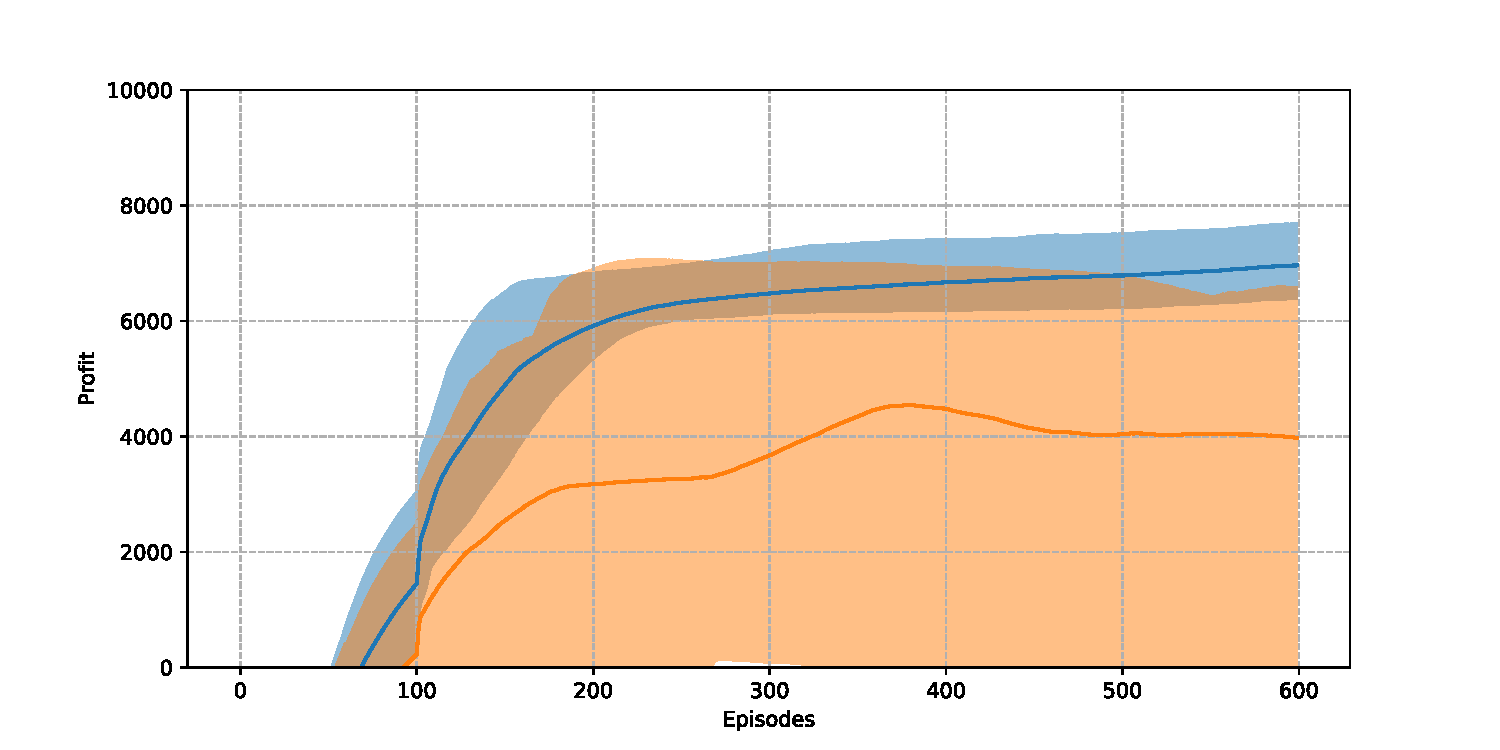
\includegraphics[width=\textwidth]{appendix/mixed_rewards_sac.pdf}
	\caption{
		Lernkurve des Soft-Actor-Critic-Algorithmus bei gemischter Rewardfunktion (orage) im Vergleich zur Standardfunktion (blau):
		Ähnlich wie bei A2C in \ref{graphic:MixedRewardsA2C} gibt es Durchläufe mit gemischter Rewardfunktion, die ähnlich zu den Durchläufen mit Standardrewardfunktion sind.
		Es gibt aber auch Durchläufe, die nie die Gewinnzone erreichen.
		Diese Durchläufe erreichen sogar bezüglich der gemischten Rewardfunktion die besten Ergebnisse, weil sie erfolgreich eine Schwäche im SAC-Algorithmus finden. (siehe \ref{graphic:ExplanationUnnormalSAC})
	}
	\label{graphic:MixedRewardsSAC}
\end{figure}
\begin{figure}[htbp]
	\centering
	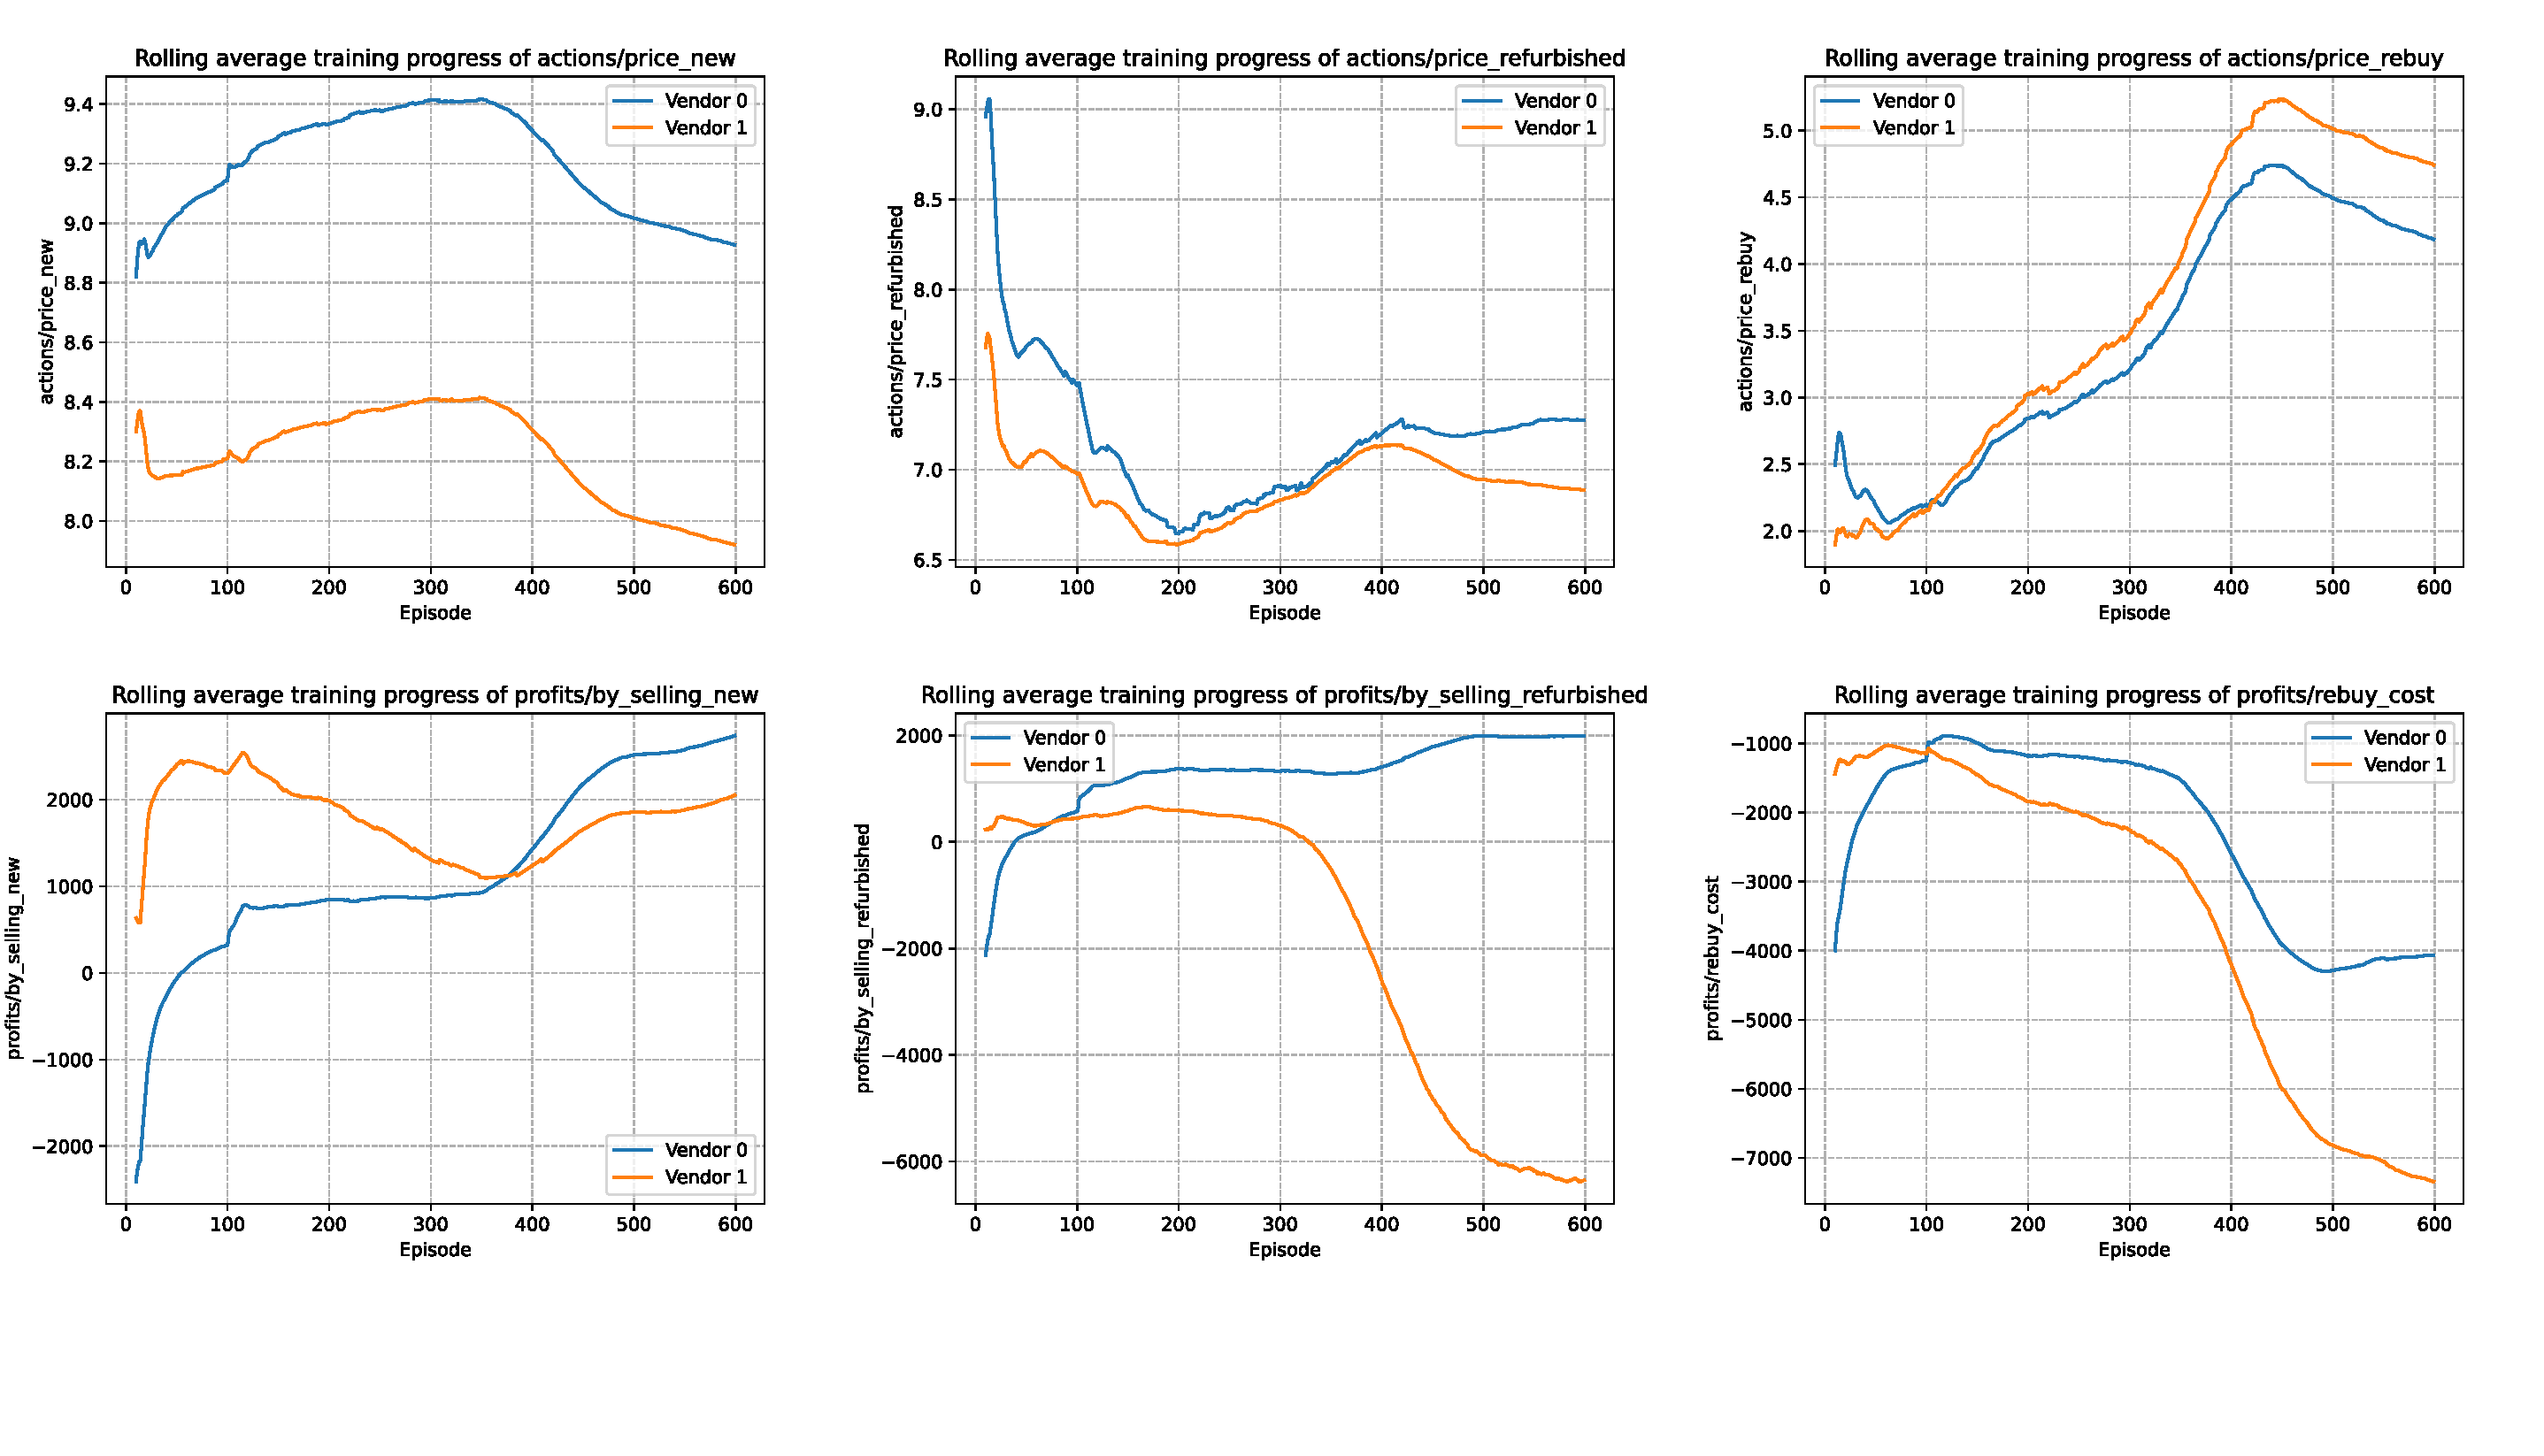
\includegraphics[width=\textwidth]{appendix/explanation_unnormal_sac.pdf}
	\caption{
		Detaillierter Blick in einen SAC-Trainingsdurchlauf gegen den regelbasierten Konkurrenten bei gemischter Rewardfunktion:
		Der SAC-Agent nutzt eine Schwäche des Konkurrenten aus und leert dessen Lager so, dass dieser Strafe für nicht bereitgestellte Produkte zahlen muss.
		Gleichzeitig versucht der regelbasierte Konkurrent, Produkte zurückzukaufen und gibt bei hohen Rückkaufpreisen dafür zu viel Geld aus.
	}
	\label{graphic:ExplanationUnnormalSAC}
\end{figure}
\begin{figure}[htbp]
	\centering
	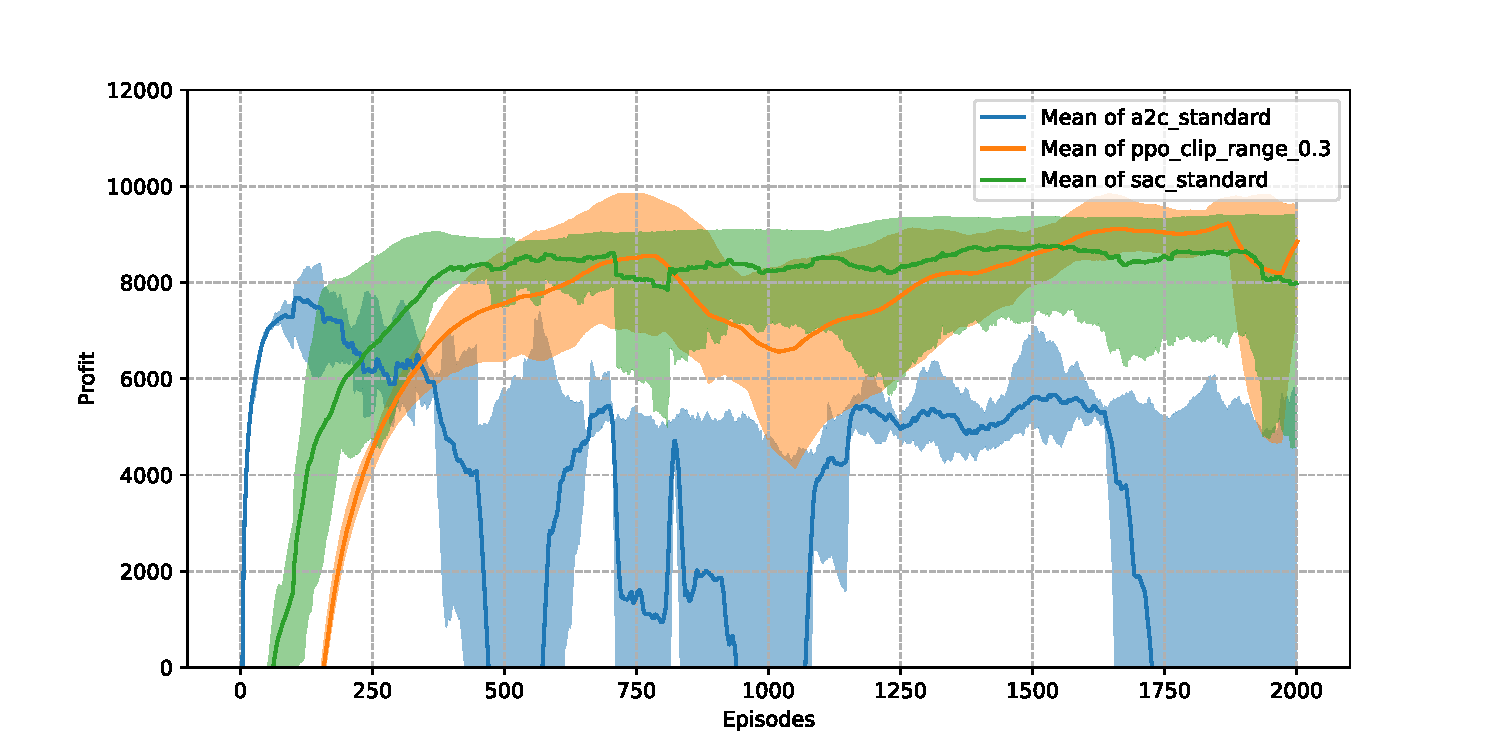
\includegraphics[width=\textwidth]{appendix/self_play_mixed.pdf}
	\caption{Lernkurve von A2C, PPO und SAC beim Self-Play bei gemischter Rewardfunktion; die Algorithmen wurden über 2000 Episoden trainiert}
	\label{graphic:SelfPlayMixedLearningCurve}
\end{figure}
\begin{figure}[htbp]
	\centering
	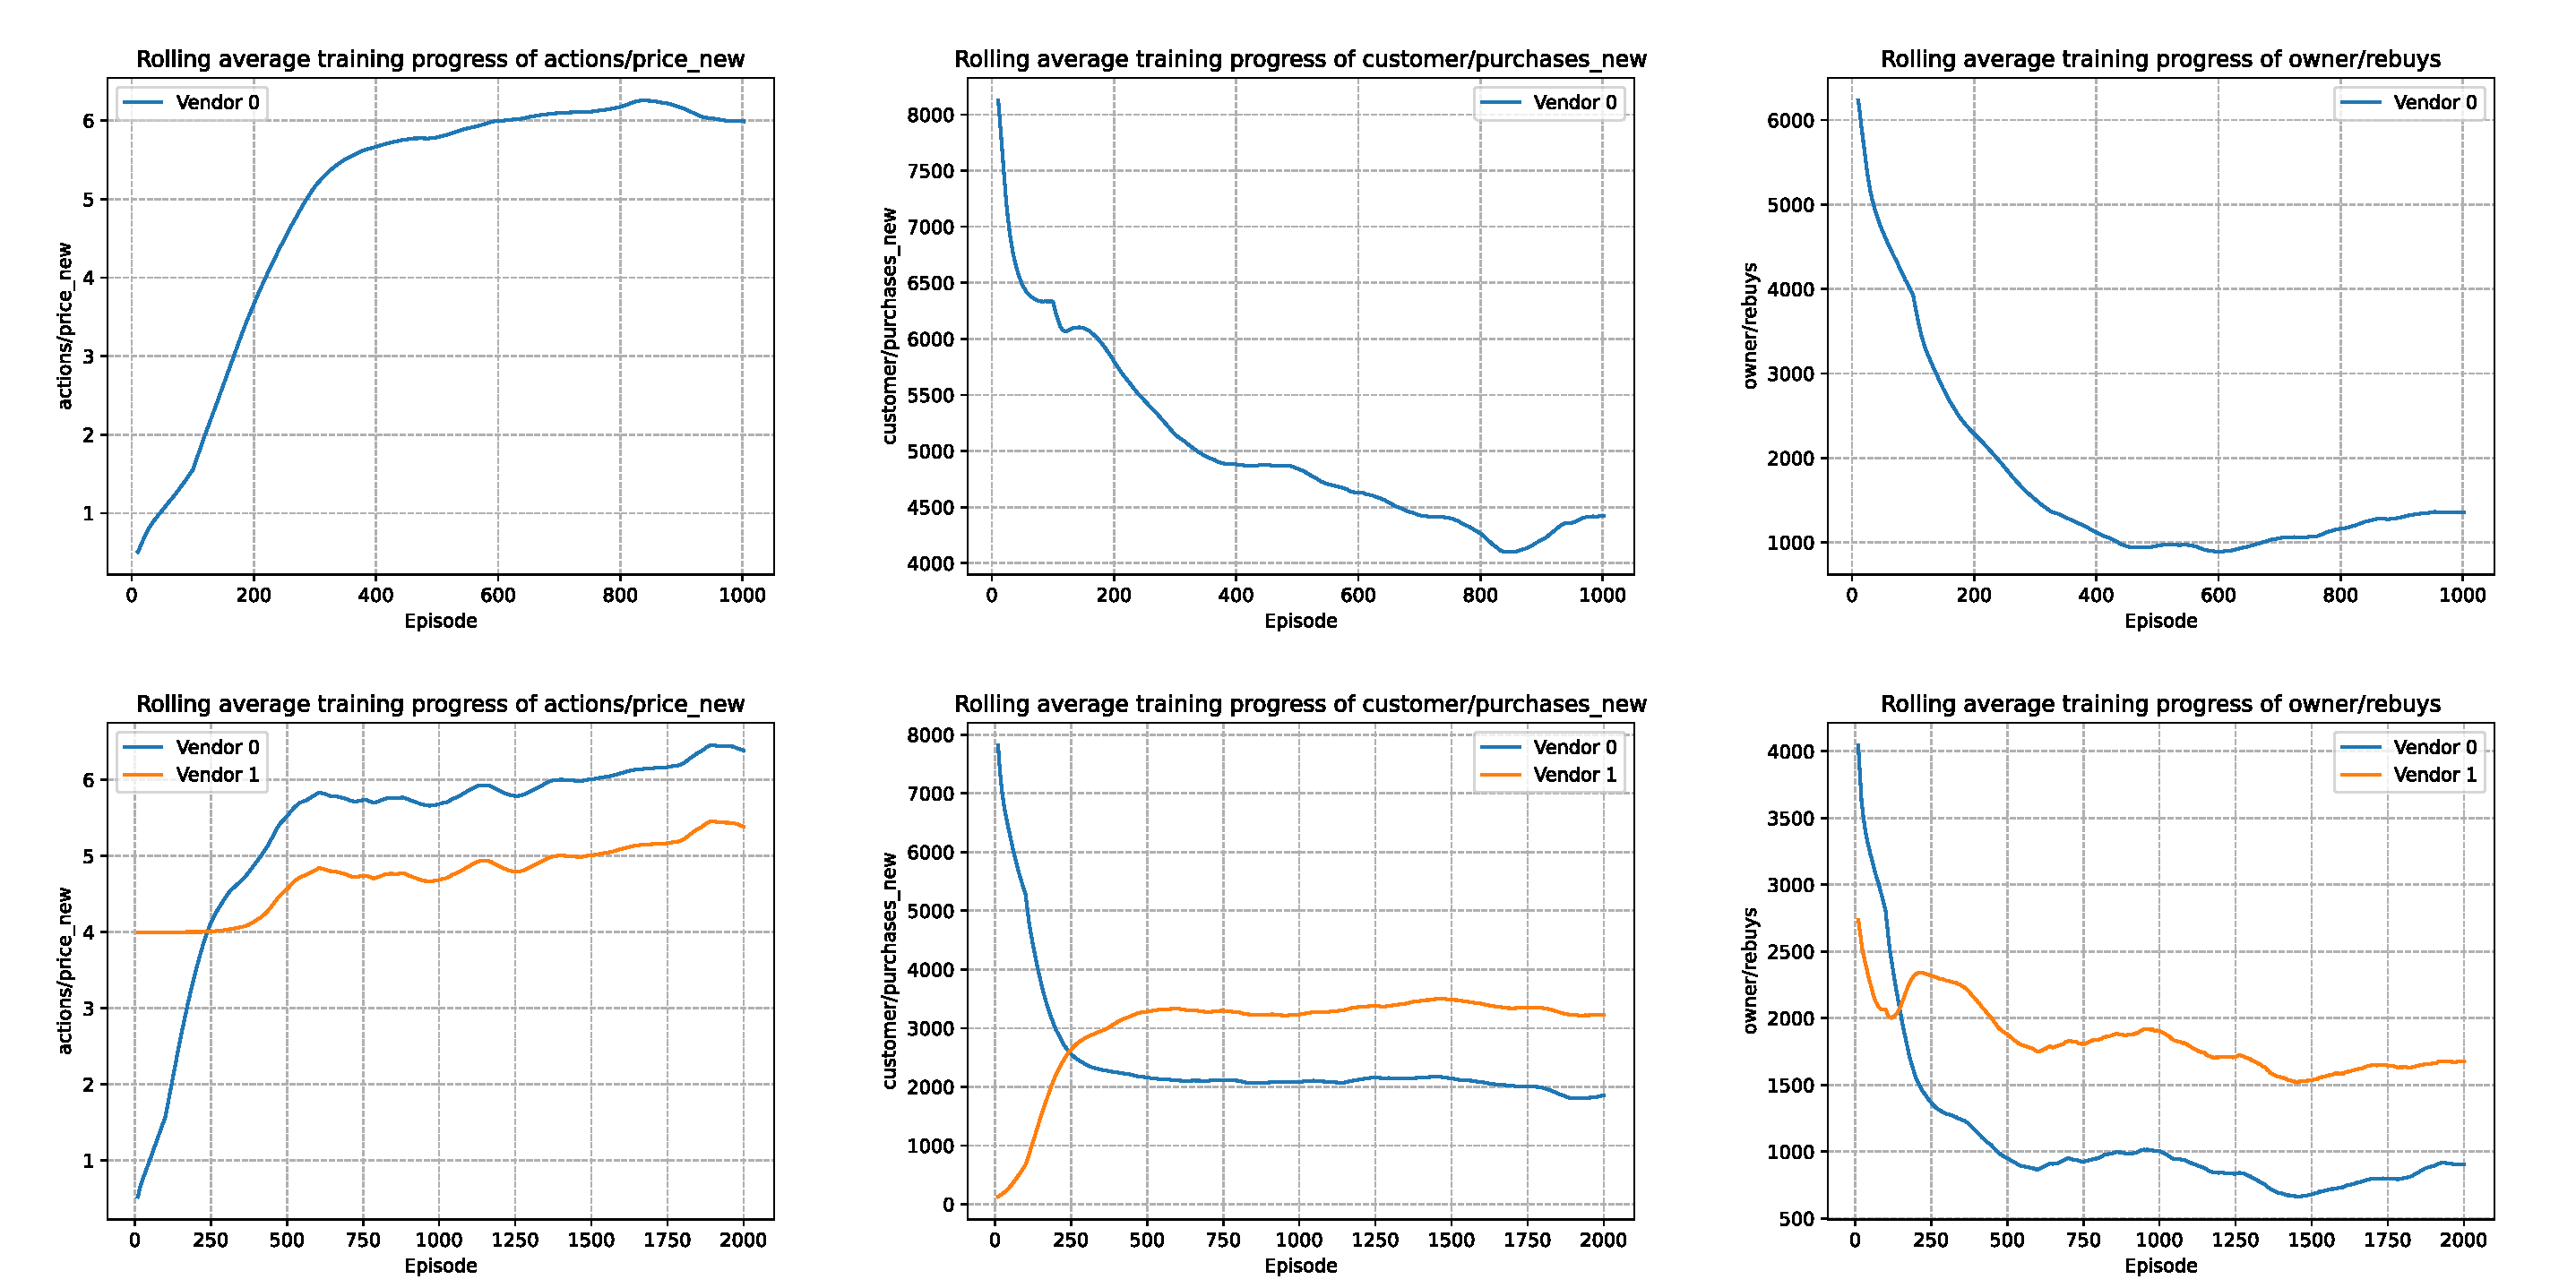
\includegraphics[width=\textwidth]{appendix/ppo_monopoly_vs_doupoly.pdf}
	\caption{
		Messungen in PPO-Trainingsdurchläufen auf einem Monopol (oben) und einem Duopol (unten):
		Dass die gesetzten Neupreise trotz Monopol nicht höher sind, liegt daran, dass die Kaufbereitschaft der Kunden mit steigenden Preisen sinkt.
		Auf dem gleichen Preisniveau verkauft der PPO-Agent im Monopol doppelt so viele Neuprodukte, die Aktivität auf dem Rebuy-Markt ist ebenfalls etwa doppelt so hoch.
	}
	\label{graphic:PPOMonopolyDuopoly}
\end{figure}